\documentclass[11pt,a4paper]{article}

\usepackage[utf8]{inputenc}
\usepackage[T1]{fontenc}
\usepackage{lmodern}
\usepackage[margin=1in]{geometry}
\usepackage{xcolor}
\usepackage{booktabs}
\usepackage{tabularx}
\usepackage{listings}
\usepackage{graphicx}
\usepackage{tikz}
\usepackage{hyperref}
\usepackage{tcolorbox}
\usepackage{enumitem}
\usepackage{caption}

% Colors
\definecolor{codegreen}{rgb}{0,0.6,0}
\definecolor{codegray}{rgb}{0.5,0.5,0.5}
\definecolor{codepurple}{rgb}{0.58,0,0.82}
\definecolor{backcolour}{rgb}{0.95,0.95,0.92}
\definecolor{primary}{RGB}{41, 128, 185}
\definecolor{secondary}{RGB}{52, 73, 94}

% Hyperref setup
\hypersetup{
    colorlinks=true,
    linkcolor=primary,
    filecolor=magenta,      
    urlcolor=primary,
    pdftitle={Pipeline Parameters Reference},
    pdfpagemode=FullScreen,
}

% Listings setup
\lstdefinestyle{mystyle}{
    backgroundcolor=\color{backcolour},   
    commentstyle=\color{codegreen},
    keywordstyle=\color{magenta},
    numberstyle=\tiny\color{codegray},
    stringstyle=\color{codepurple},
    basicstyle=\ttfamily\footnotesize,
    breakatwhitespace=false,         
    breaklines=true,                 
    captionpos=b,                    
    keepspaces=true,                 
    numbers=none,                    
    numbersep=5pt,                  
    showspaces=false,                
    showstringspaces=false,
    showtabs=false,                  
    tabsize=2
}
\lstset{style=mystyle}

% Table styling
\renewcommand{\arraystretch}{1.3}

\title{\textbf{\Huge Pipeline Parameters Reference}}
\author{Complete reference for CLI parameters across \texttt{run\_top3d.py} and \texttt{run\_pipeline.py}}
\date{}

\begin{document}

\maketitle
\tableofcontents
\newpage

\section{Quick Start Examples}

\begin{lstlisting}[language=bash, caption=Cantilever beam (150x40x4, full pipeline)]
python run_pipeline.py \
  --nelx 150 --nely 40 --nelz 4 \
  --volfrac 0.3 --penal 3.0 --rmin 3.0 --max_loop 100 \
  --load_x 150 --load_y 20 --load_z 2 \
  --load_fy -100.0 \
  --prune_len 4.15 --collapse_thresh 3.84 --rdp 0.78 \
  --radius_mode uniform --limit 5.0 --snap 5.0 \
  --visualize --output matlab_replicated.json
\end{lstlisting}

\begin{lstlisting}[language=bash, caption=Roof slab with interior columns (hybrid beam+plate)]
python run_pipeline.py \
  --problem roof_slab \
  --nelx 60 --nely 60 --nelz 40 \
  --volfrac 0.12 --penal 3.0 --rmin 2.0 --max_loop 80 \
  --load_fy -150.0 \
  --hybrid --opt_loops 2 \
  --visualize --output roof_slab.json
\end{lstlisting}

\begin{lstlisting}[language=bash, caption=Skip Top3D (reuse existing NPZ)]
python run_pipeline.py \
  --skip_top3d \
  --top3d_npz output/hybrid_v2/matlab_replicated_top3d.npz \
  --prune_len 4.15 --collapse_thresh 3.84 --rdp 0.78 \
  --visualize --output rerun.json
\end{lstlisting}

\section{\texttt{run\_top3d.py} — Standalone Top3D}

Used when you want to run topology optimisation only, producing a \texttt{.npz} file for later reconstruction.

\begin{lstlisting}[language=bash]
python run_top3d.py [OPTIONS]
\end{lstlisting}

\subsection{Domain}

\begin{table}[h]
\centering
\begin{tabularx}{\textwidth}{lllcX}
\toprule
\textbf{Parameter} & \textbf{Type} & \textbf{Default} & \textbf{Description} \\
\midrule
\texttt{--nelx} & \texttt{int} & 60 & Number of elements along X (length) \\
\texttt{--nely} & \texttt{int} & 20 & Number of elements along Y (height) \\
\texttt{--nelz} & \texttt{int} & 4 & Number of elements along Z (depth) \\
\texttt{--volfrac} & \texttt{float} & 0.3 & Target volume fraction (0.0–1.0) \\
\texttt{--penal} & \texttt{float} & 3.0 & SIMP penalty exponent. Typical: 3.0 \\
\texttt{--rmin} & \texttt{float} & 1.5 & Density filter radius. Typical: 1.5–3.0 \\
\texttt{--max\_loop} & \texttt{int} & 50 & Maximum OC optimisation iterations \\
\bottomrule
\end{tabularx}
\end{table}

\subsection{Problem Type}

\begin{table}[h]
\centering
\begin{tabularx}{\textwidth}{lllcX}
\toprule
\textbf{Parameter} & \textbf{Type} & \textbf{Default} & \textbf{Description} \\
\midrule
\texttt{--problem} & \texttt{str} & \texttt{cantilever} & Boundary condition preset. See \textbf{Problem Types}. \\
\bottomrule
\end{tabularx}
\end{table}

\subsection{Load Definition}

\begin{table}[h]
\centering
\begin{tabularx}{\textwidth}{lllcX}
\toprule
\textbf{Parameter} & \textbf{Type} & \textbf{Default} & \textbf{Description} \\
\midrule
\texttt{--load\_x} & \texttt{int} & \texttt{nelx} & X index of the load point node \\
\texttt{--load\_y} & \texttt{int} & \texttt{nely} & Y index of the load point node \\
\texttt{--load\_z} & \texttt{int} & \texttt{nelz/2} & Z index of the load point node \\
\texttt{--load\_fx} & \texttt{float} & 0.0 & Force magnitude in X direction \\
\texttt{--load\_fy} & \texttt{float} & -1.0 & Force magnitude in Y direction (downward = negative) \\
\texttt{--load\_fz} & \texttt{float} & 0.0 & Force magnitude in Z direction \\
\texttt{--load\_dist} & \texttt{str} & \texttt{point} & Distribution: \texttt{point}, \texttt{surface\_top}, \texttt{surface\_bottom} \\
\bottomrule
\end{tabularx}
\end{table}

\noindent \textbf{Load distribution modes:}
\begin{itemize}[label=--]
    \item \texttt{point} — Single node load at \texttt{(load\_x, load\_y, load\_z)}
    \item \texttt{surface\_top} — Distributed evenly across top face (\texttt{z = nelz})
    \item \texttt{surface\_bottom} — Distributed evenly across bottom face (\texttt{z = 0})
\end{itemize}

\subsection{Output}

\begin{table}[h]
\centering
\begin{tabularx}{\textwidth}{lllcX}
\toprule
\textbf{Parameter} & \textbf{Type} & \textbf{Default} & \textbf{Description} \\
\midrule
\texttt{--output} & \texttt{str} & \texttt{...result.npz} & Output file. Contains \texttt{rho}, \texttt{bc\_tags}, \texttt{pitch}, \texttt{origin} \\
\bottomrule
\end{tabularx}
\end{table}

\section{\texttt{run\_pipeline.py} — Full Pipeline}

Runs all stages: Top3D $\xrightarrow{}$ Reconstruction $\xrightarrow{}$ Size Optimisation $\xrightarrow{}$ Layout Optimisation.

\begin{lstlisting}[language=bash]
python run_pipeline.py [OPTIONS]
\end{lstlisting}

\subsection{Top3D Design Domain \& Load Definition}
Same parameters as \texttt{run\_top3d.py}. Passed directly to the Stage 0 subprocess. (\texttt{--nelx}, \texttt{--nely}, \texttt{--nelz}, \texttt{--volfrac}, \texttt{--penal}, \texttt{--rmin}, \texttt{--max\_loop}, \texttt{--load\_x/y/z}, \texttt{--load\_fx/fy/fz}, \texttt{--load\_dist}).

\subsection{Skeletonisation}

Controls how the density field from Top3D is converted into a beam skeleton.

\begin{table}[h]
\centering
\begin{tabularx}{\textwidth}{lllcX}
\toprule
\textbf{Parameter} & \textbf{Type} & \textbf{Default} & \textbf{Description} \\
\midrule
\texttt{--pitch} & \texttt{float} & 1.0 & Voxel physical size in mm. Scales geometry. \\
\texttt{--max\_iters} & \texttt{int} & 50 & Max thinning iterations for Yin's algorithm \\
\texttt{--vol\_thresh} & \texttt{float} & 0.3 & Density threshold for solid material \\
\texttt{--prune\_len} & \texttt{float} & 2.0 & Remove branches shorter than this (mm). \\
\texttt{--collapse\_thresh} & \texttt{float} & 2.0 & Collapse edges shorter than this (mm). \\
\texttt{--rdp} & \texttt{float} & 1.0 & RDP simplification epsilon (mm). 0 = off. \\
\texttt{--radius\_mode} & \texttt{str} & \texttt{uniform} & Radius estimator: \texttt{uniform} or \texttt{edt} \\
\bottomrule
\end{tabularx}
\end{table}

\begin{tcolorbox}[colback=primary!5!white,colframe=primary!75!black,title=\textbf{Tuning Guidance}]
Increase \texttt{--prune\_len} and \texttt{--collapse\_thresh} to get a cleaner, simpler graph. Decrease them to preserve finer structural details. \texttt{--rdp 0} keeps all skeleton waypoints; \texttt{--rdp 2.0} aggressively simplifies curves.
\end{tcolorbox}

\subsection{Hybrid Beam+Plate Mode}

Only active when \texttt{--hybrid} flag is set.

\begin{table}[h]
\centering
\begin{tabularx}{\textwidth}{lllcX}
\toprule
\textbf{Parameter} & \textbf{Type} & \textbf{Default} & \textbf{Description} \\
\midrule
\texttt{--hybrid} & \texttt{flag} & off & Enable hybrid beam+plate pipeline \\
\texttt{--detect\_plates} & \texttt{str} & \texttt{auto} & Detection mode: \texttt{auto}, \texttt{off}, \texttt{force} \\
\texttt{--plate\_mode} & \texttt{str} & \texttt{bspline} & Plate representation: \texttt{bspline}, \texttt{voxel}, \texttt{mesh} \\
\texttt{--plate\_thickness\_ratio}& \texttt{float} & 0.15 & Plate thickness as fraction of domain height \\
\texttt{--min\_plate\_size} & \texttt{int} & 4 & Min voxel count for plate classification \\
\texttt{--flatness\_ratio} & \texttt{float} & 3.0 & PCA eigenvalue ratio threshold. \\
\texttt{--junction\_thresh} & \texttt{int} & 4 & Neighbour count threshold for junctions \\
\texttt{--min\_avg\_neighbors} & \texttt{float} & 3.0 & Min average neighbours for plate class. \\
\bottomrule
\end{tabularx}
\end{table}

\subsection{Curved Beams (Geometry Only)}
\begin{table}[h]
\centering
\begin{tabularx}{\textwidth}{lllcX}
\toprule
\textbf{Parameter} & \textbf{Type} & \textbf{Default} & \textbf{Description} \\
\midrule
\texttt{--curved} & \texttt{flag} & off & Fits cubic Bézier curves to edges. \textbf{No FEM effect.} \\
\bottomrule
\end{tabularx}
\end{table}

\subsection{Optimisation Configuration}

\begin{table}[h]
\centering
\begin{tabularx}{\textwidth}{lllcX}
\toprule
\textbf{Parameter} & \textbf{Type} & \textbf{Default} & \textbf{Description} \\
\midrule
\texttt{--optimize} & \texttt{flag} & off & Enable beam layout/size opt (default on for beam-only) \\
\texttt{--opt\_loops} & \texttt{int} & 2 & Alternating size+layout optimisation loops \\
\texttt{--iters} & \texttt{int} & 50 & Max iterations per optimisation stage \\
\texttt{--limit} & \texttt{float} & 5.0 & Node move limit for layout opt (mm) \\
\texttt{--snap} & \texttt{float} & 5.0 & Node merge snap distance (mm) \\
\texttt{--prune\_opt\_thresh} & \texttt{float} & 0.0 & Remove edges with radius $<$ this fraction of max \\
\texttt{--problem} & \texttt{str} & \texttt{tagged} & FEM config: \texttt{tagged}, \texttt{cantilever}, \texttt{roof\_slab}, etc. \\
\bottomrule
\end{tabularx}
\end{table}

\subsection{Output, Visualisation, and Advanced}

\begin{table}[h]
\centering
\begin{tabularx}{\textwidth}{lllcX}
\toprule
\textbf{Parameter} & \textbf{Type} & \textbf{Default} & \textbf{Description} \\
\midrule
\texttt{--output} & \texttt{str} & \texttt{...beam.json} & Final output JSON filename \\
\texttt{--output\_dir} & \texttt{str} & \texttt{output/hybrid\_v2} & Directory for all stage outputs \\
\texttt{--visualize} & \texttt{flag} & off & Show 3D matplotlib debug windows \\
\texttt{--skip\_top3d} & \texttt{flag} & off & Skip Stage 0 (use existing NPZ) \\
\texttt{--top3d\_npz} & \texttt{str} & — & Path to existing NPZ (if skipping Top3D) \\
\bottomrule
\end{tabularx}
\end{table}

\section{Problem Types}

Problems define the \textbf{boundary conditions} for the topology optimisation domain. Set with \texttt{--problem}.

The domain has \texttt{(nelx+1) x (nely+1) x (nelz+1)} nodes. Coordinates: X (length), Y (height), Z (depth). All DOFs are fixed at supports unless explicitly stated.

\vspace{0.5cm}

\subsection{cantilever (default)}
A fixed-wall cantilever. The entire left face is clamped, and a point load is applied at the right.

\begin{center}
\begin{tikzpicture}[x=1cm,y=1cm]
% Wall
\fill[pattern=north east lines, pattern color=gray!50] (-0.3,0) rectangle (0,2);
\draw[thick] (0,0) -- (0,2);
% Beam
\draw[thick, fill=primary!20] (0,0) rectangle (6,2);
% Force
\draw[->, ultra thick, red] (6,1) -- (6,0) node[midway,right] {\textbf{F}};
\node at (3,1) {Domain};
\node[anchor=east] at (-0.3,1) {\shortstack{Fixed\\($x=0$)}};
\end{tikzpicture}
\end{center}

\subsection{roof}
A roof slab supported at 4 corner pillars. The 4 corner nodes at $z=0$ (inset by 1 element) are fixed. Distributed load is applied on the top surface.

\begin{center}
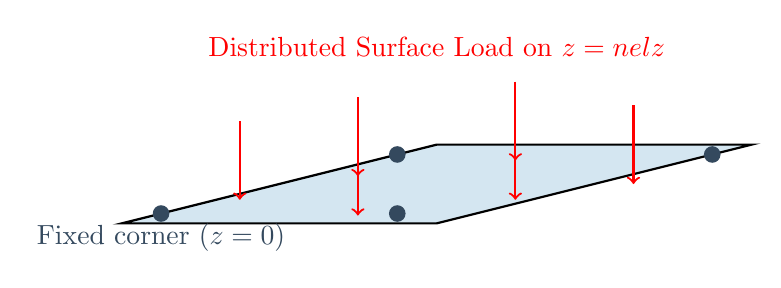
\begin{tikzpicture}[x=1cm,y=1cm]
% Top face perspective
\draw[thick, fill=primary!20] (0,0) -- (4,1) -- (8,1) -- (4,0) -- cycle;
% Uniform load
\foreach \x/\y in {1.5/0.3, 3/0.6, 5/0.8, 6.5/0.5, 3/0.1, 5/0.3} {
    \draw[->, thick, red] (\x,\y+1) -- (\x,\y);
}
\node[red, above] at (4,2) {Distributed Surface Load on $z=nelz$};
% Pillars
\fill[secondary] (0.5,0.125) circle (3pt) node[below] {Fixed corner ($z=0$)};
\fill[secondary] (3.5,0.875) circle (3pt);
\fill[secondary] (7.5,0.875) circle (3pt);
\fill[secondary] (3.5,0.125) circle (3pt);
\end{tikzpicture}
\end{center}

\subsection{roof\_slab}
A thin flat slab supported by \textbf{9 interior point columns} in a 3x3 grid. Produces a natural hybrid plate+beam decomposition.

\begin{center}
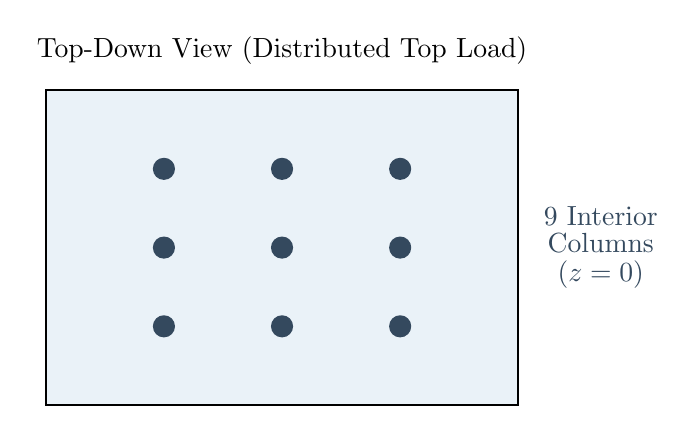
\begin{tikzpicture}[x=1cm,y=1cm]
% Top down view
\draw[thick, fill=primary!10] (0,0) rectangle (6,4);
\node at (3,4.5) {Top-Down View (Distributed Top Load)};
% Supports
\foreach \x in {1.5, 3, 4.5} {
    \foreach \y in {1, 2, 3} {
        \fill[secondary] (\x,\y) circle (4pt);
    }
}
\node[secondary, right] at (6.2, 2) {\shortstack{9 Interior\\Columns\\($z=0$)}};
\end{tikzpicture}
\end{center}

\subsection{bridge}
Bottom face fixed at ends. Suitable for simply-supported structures spanning across X.

\begin{center}
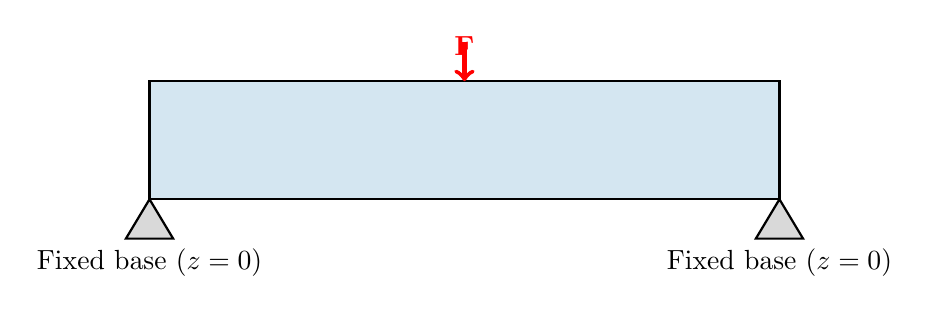
\begin{tikzpicture}[x=1cm,y=1cm]
% Beam
\draw[thick, fill=primary!20] (0,0.5) rectangle (8,2);
% Supports
\draw[thick, fill=gray!30] (0,0.5) -- (-0.3,0) -- (0.3,0) -- cycle;
\draw[thick, fill=gray!30] (8,0.5) -- (7.7,0) -- (8.3,0) -- cycle;
% Force
\draw[->, ultra thick, red] (4,2.5) -- (4,2) node[above, yshift=5pt] {\textbf{F}};
\node[below] at (0,0) {Fixed base ($z=0$)};
\node[below] at (8,0) {Fixed base ($z=0$)};
\end{tikzpicture}
\end{center}

\subsection{deck}
Entire bottom face fixed. Loads distributed at 4 top corners.

\begin{center}
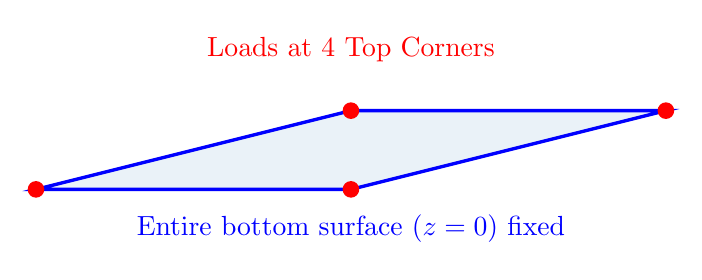
\begin{tikzpicture}[x=1cm,y=1cm]
% Domain
\draw[thick, fill=primary!10] (0,0) -- (4,1) -- (8,1) -- (4,0) -- cycle;
% Fixed base
\draw[very thick, blue] (0,0) -- (4,1) -- (8,1) -- (4,0) -- cycle;
\node[blue, below] at (4,-0.2) {Entire bottom surface ($z=0$) fixed};
% Corner loads
\fill[red] (0,0) circle (3pt);
\fill[red] (4,1) circle (3pt);
\fill[red] (8,1) circle (3pt);
\fill[red] (4,0) circle (3pt);
\node[red, above] at (4,1.5) {Loads at 4 Top Corners};
\end{tikzpicture}
\end{center}

\section{Adding a New Problem}

To define a custom problem in \texttt{run\_top3d.py}:
\begin{enumerate}
    \item Add its name to the \texttt{choices} list in the \texttt{--problem} argument.
    \item Add an \texttt{elif args.problem == "my\_problem":} block in the BC section.
    \item Use \texttt{il\_flat}, \texttt{jl\_flat}, \texttt{kl\_flat} to identify nodes.
\end{enumerate}

\begin{lstlisting}[language=python, caption=Custom BC snippet]
elif args.problem == "my_problem":
    # Fix all nodes on the right face (x = nelx)
    fixed_node_indices = np.where(il_flat == args.nelx)[0]
    fixed_dofs_list = []
    for n in fixed_node_indices:
        fixed_dofs_list.extend([3*n, 3*n+1, 3*n+2])  # fix X,Y,Z DOFs
    solver.set_fixed_dofs(np.array(fixed_dofs_list))

    # Set default load distribution if none specified
    if args.load_x is None and args.load_dist == "point":
        args.load_dist = "surface_top"
\end{lstlisting}

\section{Output Files}

\begin{table}[h]
\centering
\begin{tabularx}{\textwidth}{lX}
\toprule
\textbf{File} & \textbf{Description} \\
\midrule
\texttt{*\_top3d.npz} & Raw density field from Top3D. Arrays: \texttt{rho}, \texttt{bc\_tags}, \texttt{pitch}, \texttt{origin} \\
\texttt{*\_1\_reconstructed.json} & Skeleton graph after Stage 1. Contains nodes, edges, radii, bc\_tags \\
\texttt{*\_2\_layout.json} & Results after layout optimisation (positions updated) \\
\texttt{*\_3\_sized.json} & Results after size optimisation (radii updated) \\
\texttt{*\_history.json} & Compliance history across all optimisation loops \\
\texttt{*.json} (final) & \textbf{Final output} — use this for FreeCAD reconstruction \\
\bottomrule
\end{tabularx}
\end{table}

\end{document}
